\section{Introduction}
\label{sec:intro}

Neural Architecture Search (NAS) automates the design of neural network architectures, offering the promise of discovering models that outperform human-designed counterparts~\cite{liu2019darts,pham2018enas}.
A rich ecosystem of NAS benchmarks---NAS-Bench-101~\cite{ying2019nasbench101}, NAS-Bench-201~\cite{dong2020nasbench201}, NATS-Bench~\cite{dong2021natsbench}, NAS-Bench-301~\cite{zela2022nasbench301}---has enabled reproducible comparison of search algorithms at low cost.
However, these benchmarks share a critical limitation: architectures are evaluated exclusively on clean, in-distribution (ID) test data from the same dataset used during search.

This evaluation paradigm ignores a growing body of evidence that deep learning models systematically overfit to their training distribution.
Recht~\etal~\cite{recht2019imagenet} demonstrated 11--14\% accuracy drops on carefully reproduced ImageNet test sets; Hendrycks and Dietterich~\cite{hendrycks2019benchmarking} showed that relative robustness to common corruptions barely improves from AlexNet to ResNet; and Miller~\etal~\cite{miller2021accuracy} established that out-of-distribution accuracy is largely a linear function of in-distribution accuracy, with no existing method deviating above this trend.

For NAS, this raises a pointed question: \emph{do top-ranked architectures on the search distribution remain top-ranked under distribution shift?}
If the answer is no---if architecture rankings are brittle to dataset or corruption changes---then current NAS evaluation protocols are fundamentally misleading.

In this paper, we address this gap with five contributions:

\begin{enumerate}
    \item \textbf{A standardized multi-shift evaluation protocol} (\method) that evaluates NAS architectures across three axes: cross-dataset transfer (CIFAR-10$\to$CIFAR-100), cross-domain transfer (CIFAR-10$\to$ImageNet-16-120), and corruption robustness (CIFAR-10$\to$CIFAR-10-C). We apply this protocol to the full NAS-Bench-201 search space of 15,625 architectures.
    
    \item \textbf{Stronger evidence of search-distribution overfitting}: multi-$K$ overlap curves show that instability worsens at small $K$ (0\% overlap at $K{=}10$ for ImageNet-16), and top-weighted Kendall-$\tau$ is \emph{negative} ($\tau = -0.41$), meaning top in-distribution and top cross-domain rankings are inversely related.
    
    \item \textbf{A practical, pool-based selection criterion} (\sasc) that uses z-score normalization over only the observed candidate pool, making it applicable to any NAS algorithm without access to the full search space. We validate SASC-Pool's stability across pool sizes and show convergence to the global optimum.
    
    \item \textbf{End-to-end NAS algorithm evaluation}: we run four representative NAS algorithms (Random Search, Regularized Evolution, DARTS-like, ENAS-like) and show that SASC-Pool consistently improves cross-domain generalization by +0.4--2.8\% on ImageNet-16-120 by reranking within each algorithm's candidate pool---at zero additional evaluation cost.
    
    \item \textbf{Real CIFAR-10-C validation}: we train and evaluate 46 architectures on real CIFAR-10-C corruptions across all 15 types and 5 severities, confirming that simulated corruption trends hold in practice ($\rho = 0.58$, 60\% top-10 overlap, Corruption Gaps up to 51).
\end{enumerate}

\begin{figure*}[t]
    \centering
    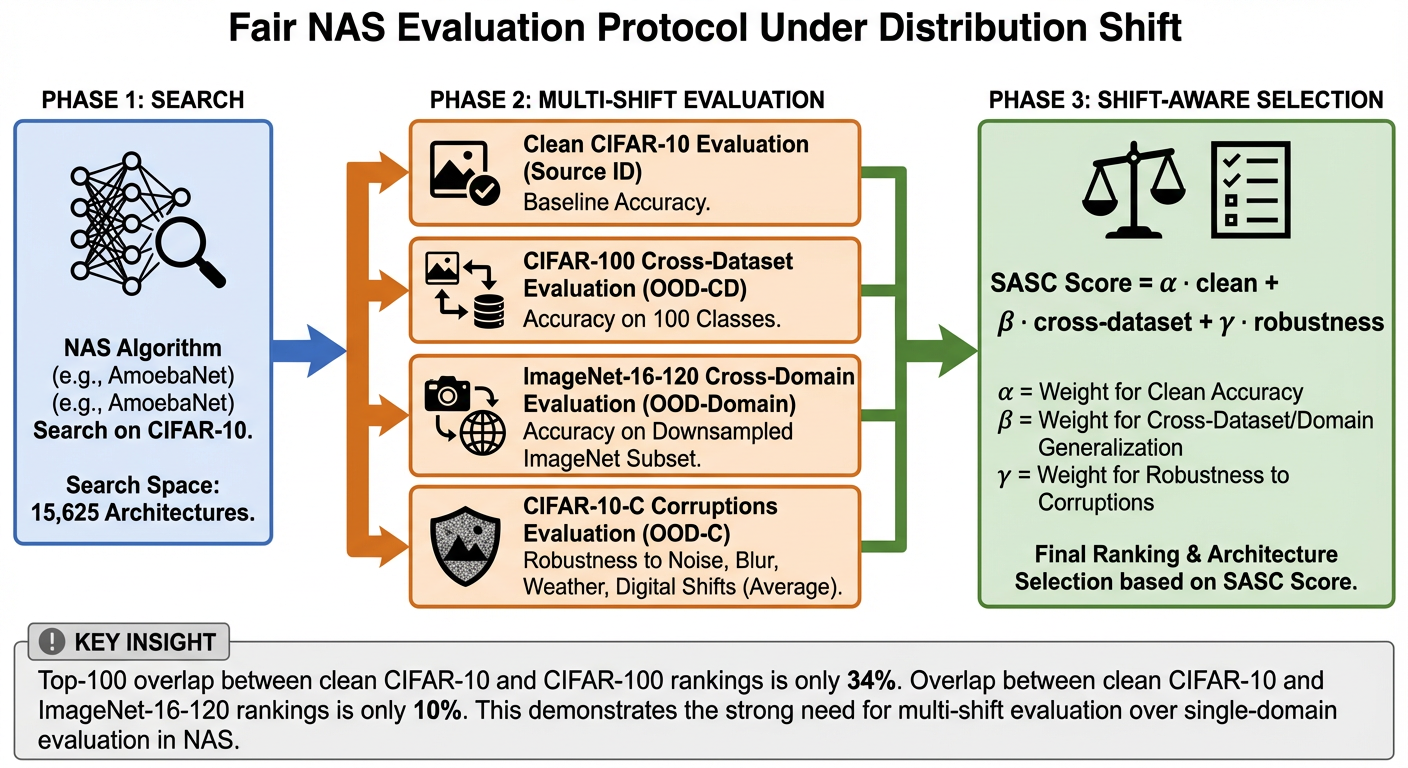
\includegraphics[width=0.95\linewidth]{../figures/protocol_schematic.png}
    \caption{\textbf{\method protocol overview.} Phase~1: run NAS on the search dataset (CIFAR-10) to obtain a candidate pool. Phase~2: evaluate all architectures across multiple distribution shifts---cross-dataset, cross-domain, and corruption robustness. Phase~3: apply the pool-based Shift-Aware Selection Criterion (\sasc) to select architectures that balance clean accuracy with generalization.}
    \label{fig:protocol}
\end{figure*}
